\section{单层重述}
\label{sec:bilevel-single-level}

前两节都把$\Phi$当作函数，靠内层求解和求导来下降。另一种思路是不把内层嵌套着解，而把“$\bm{y}$确实是内解”写成关于$(\bm{x},\bm{y})$的约束，然后一起最小化外层目标。接下来要弄清：这样的约束有哪些写法，每种写法保留了什么，又失去了什么？

对乐观模型，由式~\eqref{eq:bilevel-optimistic-joint}，这个想法可以直接实现。悲观模型不行：外层目标里夹着一个对解集的$\sup$，把它改成对$\bm{y}$的联合最小化就等于把最坏情况换成了最好情况，它还需要再嵌套一层，不能套用下面的改写。本节只讨论乐观模型。

\subsection{最优性条件重述}
\label{sec:bilevel-kkt-reformulation}

用$\bm{y}$的最优性条件替代“$\bm{y}\in\bm{S}(\bm{x})$”是最直接的做法，内层有约束时这就是KKT条件。

\paragraph{写成一个单层问题}
沿用式~\eqref{eq:bilevel-lagrangian}的记号，把乘子也作为变量，得到下面的问题：
\begin{equation}
 \begin{aligned}
 \min_{\bm{x},\bm{y},\bm{\lambda},\bm{\nu}}\quad&F(\bm{x},\bm{y})\\
 \text{s.t.}\quad&\bm{x}\in\bm{C},\quad\nabla_{\bm{y}}\mathcal{L}=\bm{0},\quad\bm{h}=\bm{0},\\
 &\bm{c}\leq\bm{0},\quad\bm{\lambda}\geq\bm{0},\quad\lambda_ic_i=0,\ i=1,\ldots,m.
 \end{aligned}
 \label{eq:bilevel-mpcc}
\end{equation}
含有$\lambda_ic_i=0$这样的约束的问题称为\term{互补约束规划}（mathematical program with complementarity constraints），简称MPCC。

这样的改写要成立，必须保证KKT条件恰好刻画内层的全局解。KKT条件一般只是局部解的必要条件，下面的定理给出能作此替换的情形。

\begin{theorem}[凸内层的KKT重述]
\label{thm:bilevel-kkt-equivalence}
设对每个$\bm{x}\in\bm{C}$，$g(\bm{x},\cdot)$和$c_i(\bm{x},\cdot)$凸且连续可微，$h_j(\bm{x},\cdot)$仿射，内层满足Slater条件。则对每个$\bm{x}\in\bm{C}$，
\begin{equation}
 \bm{y}\in\bm{S}(\bm{x})\iff\text{存在}(\bm{\lambda},\bm{\nu})\text{使}(\bm{x},\bm{y},\bm{\lambda},\bm{\nu})\text{满足式~\eqref{eq:bilevel-mpcc}的约束}.
 \label{eq:bilevel-kkt-equivalence}
\end{equation}
于是$(\bm{x},\bm{y})$是乐观模型的全局解，当且仅当存在乘子使$(\bm{x},\bm{y},\bm{\lambda},\bm{\nu})$是式~\eqref{eq:bilevel-mpcc}的全局解。
\end{theorem}

\begin{proof}
固定$\bm{x}$。凸问题的KKT点是全局解，这给出“$\Leftarrow$”；Slater条件下凸问题的全局解满足KKT条件，乘子存在，这给出“$\Rightarrow$”。这两个结论见第~\ref{chap:constrained-optimality}章和第~\ref{chap:duality}章。两个问题的目标都只含$(\bm{x},\bm{y})$，可行点的$(\bm{x},\bm{y})$分量又相同，所以全局解的$(\bm{x},\bm{y})$分量也相同。
\end{proof}

定理只对应全局解。局部解的对应要复杂得多：式~\eqref{eq:bilevel-mpcc}的局部解固定了一组乘子，而原问题要比较所有乘子对应的邻近点，乘子不唯一时两者可以不一致。相关反例的构造较长，读者可查阅双层规划的专门文献。

\paragraph{非凸内层的反例}
内层非凸时，KKT点可能根本不是全局解。取无约束内层和外层
\[
 g(y)=\frac14y^4-\frac12y^2,\qquad F(y)=\frac12y^2.
\]

驻点方程$y^3-y=0$的解是$y\in\{-1,0,1\}$。全局解是$y=\pm1$，外层值是$1/2$。可是重述问题只要求驻点方程，它会选$y=0$，外层值是$0$，而$y=0$恰好是内层的局部极大点。

\paragraph{一个凸内层的例子}
取内层$\min_y\frac12(y-x)^2$，约束$y\geq0$，也就是$c=-y\leq0$。外层目标取$F=\frac12(x+1)^2+\frac12(y-1)^2$。内层的KKT条件是
\[
 y-x-\lambda=0,\qquad y\geq0,\qquad\lambda\geq0,\qquad\lambda y=0.
\]

互补条件把可行集分成两支。$\lambda=0$时$y=x\geq0$；$y=0$时$\lambda=-x\geq0$。这就是图~\ref{fig:bilevel-mpcc}(b)的折线，$y^\star(x)=\max\{x,0\}$。

在两支上分别求解。沿$y=x$，$x\geq0$，外层值是$x^2+1$，最小值是$x=0$处的$1$。沿$y=0$，$x\leq0$，外层值是$\frac12(x+1)^2+\frac12$，最小值是$x=-1$处的$\frac12$。全局解是$(x,y)=(-1,0)$。

\paragraph{互补约束为什么难}
图~\ref{fig:bilevel-mpcc}(a)画出了$a\geq0$、$b\geq0$、$ab=0$的可行集，它由两条半轴组成，没有内部，在原点还拐了一个直角。一般非线性规划算法依靠约束资格，而这类可行集恰好破坏它们。

\begin{BookInlineFigure}
 \centering
 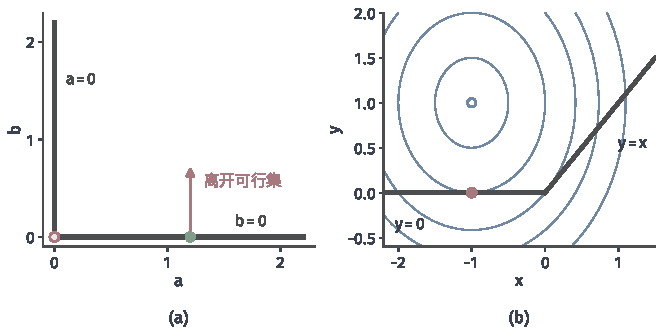
\includegraphics[width=112mm]{figures/05-optimization/07-multiple-criteria-and-nested-optimization/matplotlib/bilevel-mpcc/figure.pdf}
 \caption{互补约束的几何。(a)$a\geq0$、$b\geq0$、$ab=0$的可行集是两条半轴。在绿点处，严格满足不等式$b\geq0$的方向（红箭头）立刻离开可行集；原点处（空心点）拐角使等式约束的梯度为零。(b)内层$\min\frac12(y-x)^2$，$y\geq0$的解图像（深灰折线），蓝色是外层等高线，空心点是外层的无约束最小点$(-1,1)$，红点是双层问题的解$(-1,0)$。}
 \label{fig:bilevel-mpcc}
\end{BookInlineFigure}

\begin{lemma}[互补约束破坏MFCQ]
\label{lem:bilevel-mfcq-fails}
设$m\geq1$。式~\eqref{eq:bilevel-mpcc}的每个可行点都不满足Mangasarian—Fromovitz约束资格（MFCQ）。
\end{lemma}

\begin{proof}
MFCQ要求等式约束的梯度线性无关，并存在方向$\bm{d}$，使它与所有等式约束的梯度正交，且与所有活动不等式约束的梯度内积为负。考虑某一对约束$\lambda_i\geq0$、$c_i\leq0$、$e=\lambda_ic_i=0$，在全部变量构成的空间中，等式的梯度是
\[
 \nabla e=c_i\nabla\lambda_i+\lambda_i\nabla c_i.
\]

若$\lambda_i>0$，$c_i=0$，则$\nabla e=\lambda_i\nabla c_i$。$c_i\leq0$活动，MFCQ要求$\langle\nabla c_i,\bm{d}\rangle<0$，于是$\langle\nabla e,\bm{d}\rangle<0$，与正交矛盾。

若$\lambda_i=0$，$c_i<0$，则$\nabla e=c_i\nabla\lambda_i$。$-\lambda_i\leq0$活动，MFCQ要求$\langle\nabla\lambda_i,\bm{d}\rangle>0$，于是$\langle\nabla e,\bm{d}\rangle<0$，同样矛盾。

若$\lambda_i=c_i=0$，则$\nabla e=\bm{0}$，等式约束的梯度线性相关。三种情形穷尽了可行点的所有可能。
\end{proof}

所以即使内层是凸的，也不能把一般非线性规划的收敛结论直接搬过来，那些结论通常要求某种约束资格。实践中的做法有两类：内层约束不多时枚举互补的分支，每一支是一个正常的问题，但分支数最多是$2^m$；或者把$\lambda_ic_i=0$松弛成$-\lambda_ic_i\leq t$，让$t$逐渐趋于零，松弛问题有内部，但收敛到的点要回到原问题核对。

\subsection{值函数重述}
\label{sec:bilevel-value-reformulation}

最优性条件的重述要靠凸性才能表达全局最优。另一种写法直接比较目标值，不需要内层的结构。

\paragraph{直接比较内层目标值}
定义内层最优值函数
\begin{equation}
 V(\bm{x})=\inf_{\bm{y}\in\bm{Y}(\bm{x})}g(\bm{x},\bm{y}).
 \label{eq:bilevel-value-function}
\end{equation}
$\bm{y}$是内解，当且仅当它内层可行，且它的内层目标值达到了最优值。

\begin{lemma}[值函数重述]
\label{lem:bilevel-value-reformulation}
设$V(\bm{x})$有限。则
\begin{equation}
 \bm{y}\in\bm{S}(\bm{x})\iff\bm{y}\in\bm{Y}(\bm{x})\text{且}g(\bm{x},\bm{y})\leq V(\bm{x}).
 \label{eq:bilevel-value-constraint}
\end{equation}
\end{lemma}

\begin{proof}
若$\bm{y}\in\bm{S}(\bm{x})$，则$\bm{y}$可行且$g(\bm{x},\bm{y})=V(\bm{x})$。反过来，$\bm{y}$可行时必有$g(\bm{x},\bm{y})\geq V(\bm{x})$，再加上不等式$g(\bm{x},\bm{y})\leq V(\bm{x})$，就得到等号，所以$\bm{y}$取得内层最小值。
\end{proof}

引理没有用到任何凸性，所以全局选解这个要求被完整地写了下来。乐观模型因而等价于
\[
 \min_{\bm{x}\in\bm{C},\,\bm{y}\in\bm{Y}(\bm{x})}F(\bm{x},\bm{y})\quad\text{s.t.}\quad g(\bm{x},\bm{y})-V(\bm{x})\leq0.
\]

\paragraph{用正则拟合例计算}
把式~\eqref{eq:bilevel-ridge-solution}代入$g$并化简，得到
\[
 V(x)=\frac{9x}{2(1+x)}.
\]

$g$对$y$是二次函数，二次项系数为$(1+x)/2$，所以
\[
 g(x,y)-V(x)=\frac{1+x}{2}\bigl(y-y^\star(x)\bigr)^2.
\]
约束$g-V\leq0$迫使$y=y^\star(x)$，确实把内解曲线重新写了出来。$V$的导数可以用包络关系求，
\[
 V'(x)=\partial_xg(x,y^\star(x))=\frac12(y^\star)^2=\frac{9}{2(1+x)^2},
\]
它和直接求导的结果相同。

\paragraph{两个困难}
第一，$V$可能不光滑。式~\eqref{eq:bilevel-two-wells}的内层有$V(x)=-\lvert x\rvert$，在切换点$x=0$处有折点，如图~\ref{fig:bilevel-value}(a)。一般地，$V$是一族函数的下确界，切换解的地方就会出现折点。计算$V$本身也要解一次内层问题。

第二，约束本身是退化的。在$\bm{y}\in\bm{Y}(\bm{x})$上总有$g-V\geq0$，所以不存在严格满足$g-V<0$的点，Slater条件永远不成立。上面的例子里更明显：约束函数$\frac{1+x}{2}(y-y^\star)^2$在可行点处的梯度是零向量，它提供不了任何关于如何回到可行集的一阶信息。

\paragraph{松弛之后要重新核对}
常见的处理是把约束放宽成$g-V\leq\varepsilon$，$\varepsilon>0$。这样可行集有了内部，但代价是允许了不是内解的点。

正则拟合例中，$\varepsilon=0.1$时可行集成了内解曲线周围的一条带，它的半宽是$\sqrt{2\varepsilon/(1+x)}$，见图~\ref{fig:bilevel-value}(b)。外层目标在$y=1$处取最小值$0$，带子与直线$y=1$相交的部分全部是松弛问题的解。令$u=1+x$，条件是
\[
 (u-3)^2\leq0.2\,u.
\]

解得$u\in[2.319,3.881]$，即$x\in[1.319,2.881]$。真实的解$x=2$只是其中一点，松弛让最优解从一个点变成了一个区间，最优值也可能偏低。

\begin{BookInlineFigure}
 \centering
 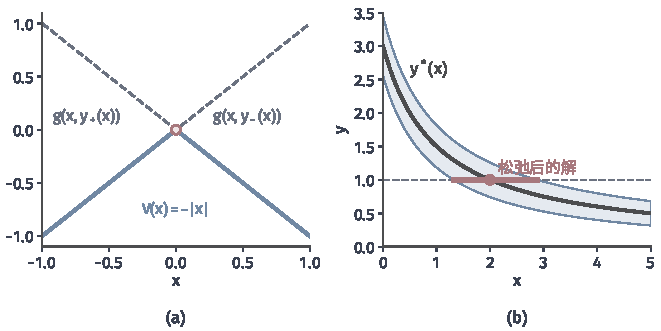
\includegraphics[width=112mm]{figures/05-optimization/07-multiple-criteria-and-nested-optimization/matplotlib/bilevel-value/figure.pdf}
 \caption{值函数重述的两个困难。(a)式~\eqref{eq:bilevel-two-wells}的最优值函数$V(x)=-|x|$（蓝），虚线是沿两条分支的内层值，切换点（空心点）处$V$不可微。(b)正则拟合例的松弛$g-V\leq0.1$：浅蓝带是松弛后的可行集，深灰线是内解，红色线段是带子与$y=1$的交集，即松弛问题的全部最优解；红点是原问题的解$x=2$。}
 \label{fig:bilevel-value}
\end{BookInlineFigure}

罚函数也可以用，把$\rho(g-V)$加进外层目标。有限的$\rho$得到的通常只是近似解。不论松弛还是惩罚，得到的点都要重新检查：内层最优间隙$g-V$有多大，它对应的内解距离有多大，以及改变$\varepsilon$或$\rho$后解是否稳定。

表~\ref{tab:bilevel-reformulations}比较两种重述。

\begin{BookInlineTable}
 \centering
 \begin{tabular}{lll}
  \toprule
  & KKT重述 & 值函数重述\\
  \midrule
  全局等价 & 需凸性与约束资格 & 不需要\\
  新增变量 & 乘子 & 无\\
  主要困难 & 互补约束 & $V$的计算与不光滑\\
  约束资格 & MFCQ处处失效 & Slater永不成立\\
  \bottomrule
 \end{tabular}
 \caption{乐观模型的两种单层重述。悲观模型不能这样改写。}
 \label{tab:bilevel-reformulations}
\end{BookInlineTable}
